\documentclass[conference,letterpaper]{IEEEtran}
\IEEEoverridecommandlockouts
% Camera-ready: if the conference supplies a copyright notice, uncomment and fill in:
% \IEEEpubid{\makebox[\columnwidth]{979-8-XXXX-XXXX-X/XX/\$31.00~\copyright2026 IEEE \hfill}\hspace{\columnsep}\makebox[\columnwidth]{ }}

\usepackage{cite}
\usepackage{amsmath}
\usepackage{newtxtext,newtxmath}
\usepackage{graphicx}
\usepackage{booktabs}
\usepackage{multirow}
\usepackage{tikz}
\usetikzlibrary{positioning,arrows.meta}
\usepackage{balance}
\usepackage[hidelinks]{hyperref}

\newcommand{\tA}{\tau_A}
\newcommand{\tC}{\tau_C}

\begin{document}

\title{Evidence-Calibrated Enterprise RAG for\\Hallucination-Resistant Question Answering}

\author{\IEEEauthorblockN{Abayomi Adelowotan}
\IEEEauthorblockA{Chevron\\Lagos, Nigeria\\abayomi.adelowotan@chevron.com}
\and
\IEEEauthorblockN{Kikelomo Obayemi}
\IEEEauthorblockA{Chevron\\Lagos, Nigeria\\liim@chevron.com}}

\maketitle

\begin{abstract}
Retrieval-augmented generation (RAG) reduces but does not remove unsupported answers in
enterprise question answering, where evidence may be incomplete, contradictory, or outdated.
We study Evidence-Calibrated Enterprise RAG (ECERAG), a selective answering framework that scores
the sufficiency of retrieved evidence from four signals---relevance, coverage, agreement, and
source trust/recency---and answers, asks for clarification, or abstains accordingly. We evaluate it
on a 60-question benchmark built from SEC filings, the NIST AI Risk Management Framework, the
OWASP Top~10, and current/obsolete IETF specifications, under clean retrieval and three
perturbations (irrelevant, contradictory, and outdated evidence), with five open-weight generators
from 0.5B to 14B parameters, repeated cross-validation, paired bootstrap intervals, and two
independent graders. Relative to a RAG baseline that must always answer, ECERAG cuts the error
rate on answered questions by roughly two-thirds (e.g., 0.43 to 0.13 at 7B; 0.40 to 0.11 at 14B).
A controlled decomposition shows that most of this gain comes from the generator's own
evidence-grounded refusal; the external sufficiency gate alone yields small reductions (at most
0.01--0.11), significant only for the 7B model or under outdated evidence. The sufficiency score is
nevertheless a reliable ranking signal: among answered questions it orders wrong answers below
right ones better than chance at every generator size from 1.5B to 14B. We conclude that
\emph{retrieve--assess--decide} is effective, that assessment is best led by grounded
self-refusal, and that evidence-side scores are a complementary confidence signal rather than a
standalone defense.
\end{abstract}

\begin{IEEEkeywords}
retrieval-augmented generation, hallucination, selective prediction, calibration,
enterprise question answering, trustworthy AI
\end{IEEEkeywords}

\section{Introduction}
Enterprise deployments of large language models (LLMs) need factual reliability and auditable
behavior under uncertainty: in financial, legal, and engineering settings a confident wrong
answer can cause material harm. Retrieval-augmented generation (RAG) grounds answers in retrieved
documents~\cite{lewis2020rag,gao2023survey}, but a standard pipeline still answers
unconditionally, even when the retrieved passages are irrelevant, contradictory, or superseded.

ECERAG makes answering conditional on an explicit assessment of the evidence. A sufficiency score
$S(q,E)$ routes each query to \emph{Answer}, \emph{Clarify}, or \emph{Abstain}, in the tradition of
selective prediction~\cite{geifman2019selectivenet,kamath2020selective}. Our research question is:
\emph{can evidence-sufficiency signals reduce unsupported answers in enterprise RAG without
materially degrading coverage, and how much of any reduction is due to the evidence gate itself?}

A pilot of this design with 40 questions and a 0.5B-parameter generator found no reduction in
selective risk, and attributed most errors to the generator. This paper replaces that pilot with a
controlled study and makes four contributions:
\begin{enumerate}
\item A fully specified sufficiency score and selective policy (Sec.~\ref{sec:method}), including
a conflict check that detects near-duplicate passages disagreeing on a figure.
\item A generator-scale study (0.5B--14B) with repeated cross-validation, so every question is a
held-out test item, and paired bootstrap confidence intervals (Sec.~\ref{sec:setup}).
\item A decomposition that separates the evidence gate from the generator's own refusal by adding
a truly unconditional baseline and a gate-only system (Sec.~\ref{sec:decomp}).
\item Evidence that the sufficiency score is a reliable \emph{ranking} signal for answer
correctness across scales, even where thresholded gating adds little (Sec.~\ref{sec:ranking}).
\end{enumerate}

\section{Related Work}
\textbf{Retrieval-augmented generation.} RAG couples a parametric generator with non-parametric
retrieval~\cite{lewis2020rag}, building on dense retrieval~\cite{karpukhin2020dpr},
late interaction~\cite{khattab2020colbert}, and fusion-in-decoder
readers~\cite{izacard2021fid}; surveys document persistent failures under weak or noisy
retrieval~\cite{gao2023survey}. \textbf{Adaptive and corrective retrieval.}
Self-RAG~\cite{asai2023selfrag} trains the generator to retrieve and critique on demand;
Corrective RAG~\cite{yan2024crag} detects poor retrieval and re-retrieves. Neither defines an
explicit abstention policy calibrated to enterprise risk. \textbf{Selective prediction.} A
selective model trades coverage for lower risk on the inputs it accepts~\cite{elyaniv2010,geifman2019selectivenet};
Kamath et al.~\cite{kamath2020selective} apply this to QA under domain shift, and LLMs have been
shown to partly know what they know~\cite{kadavath2022know}---a point our decomposition makes
concrete for RAG. \textbf{Evaluation.} RAG evaluation has moved toward faithfulness and context
relevance~\cite{es2023ragas}, robustness to retrieval shift~\cite{thakur2021beir}, and
attribution~\cite{bohnet2022attributed}; LLM-as-judge grading~\cite{zheng2023judge} is
increasingly used and should be cross-checked, as we do here.

\section{Method}\label{sec:method}
\begin{figure*}[t]
\centering
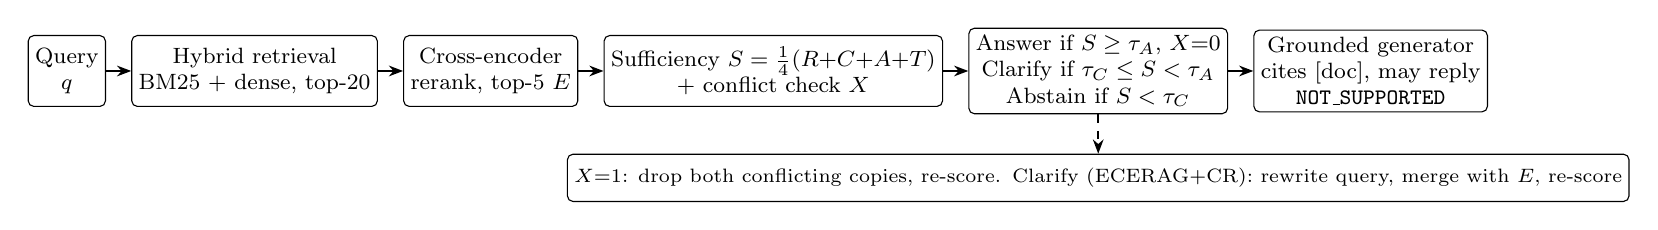
\begin{tikzpicture}[
  box/.style={draw, rounded corners=2pt, align=center, font=\footnotesize, minimum height=9mm, inner sep=2.5pt},
  arr/.style={-{Stealth[length=1.8mm]}, thick}, node distance=3.2mm]
\node[box] (q) {Query\\$q$};
\node[box, right=of q] (ret) {Hybrid retrieval\\BM25 + dense, top-20};
\node[box, right=of ret] (rr) {Cross-encoder\\rerank, top-5 $E$};
\node[box, right=of rr] (s) {Sufficiency $S=\tfrac14(R{+}C{+}A{+}T)$\\+ conflict check $X$};
\node[box, right=of s] (pol) {Answer if $S\ge\tA$, $X{=}0$\\Clarify if $\tC\le S<\tA$\\Abstain if $S<\tC$};
\node[box, right=of pol] (gen) {Grounded generator\\cites [doc], may reply\\\texttt{NOT\_SUPPORTED}};
\draw[arr] (q) -- (ret); \draw[arr] (ret) -- (rr); \draw[arr] (rr) -- (s); \draw[arr] (s) -- (pol); \draw[arr] (pol) -- (gen);
\node[box, below=5mm of pol, font=\scriptsize, minimum height=6mm] (cr) {$X{=}1$: drop both conflicting copies, re-score.\enspace Clarify (ECERAG+CR): rewrite query, merge with $E$, re-score};
\draw[arr, dashed] (pol.south) -- (cr.north);
\end{tikzpicture}
\caption{ECERAG pipeline. Every component is specified in Sec.~\ref{sec:method}.}
\label{fig:pipeline}
\end{figure*}

\subsection{Retrieval}
Documents are split into 220-word passages with a 40-word overlap. For a query $q$, BM25~\cite{robertson2009bm25}
scores and cosine similarities of \texttt{all-MiniLM-L6-v2} embeddings~\cite{reimers2019sbert} are
each min--max normalized over the corpus and averaged with equal weight. The top 20 passages are
reranked with the \texttt{ms-marco-MiniLM-L-6-v2} cross-encoder~\cite{devlin2019bert}, and the top
five form the evidence set $E=\{e_1,\dots,e_5\}$.

\subsection{Evidence Sufficiency Score}
$S(q,E)=\tfrac14(R+C+A+T)\in[0,1]$, with equal weights (fitting the weights did not help at this
data size; Sec.~\ref{sec:ablation}).

\emph{Relevance} $R$ is the mean cross-encoder probability $\sigma(\ell_i)$ over $E$, where
$\ell_i$ is the reranker logit for $(q,e_i)$.

\emph{Coverage} $C$ is the fraction of the query's salient terms (lower-cased alphanumeric tokens
of at least three characters, excluding stop words) that occur in the concatenated evidence.

\emph{Agreement} $A$ is the mean over passage pairs $(i,j)$ of the embedding cosine similarity
$s_{ij}$, multiplied by $0.1$ when the pair conflicts. Let $N_i$ be the set of numbers in $e_i$.
A pair conflicts if it is on the same topic ($s_{ij}>0.55$) and $N_i\cap N_j=\emptyset$, or if both
passages come from the same document, are near-duplicates ($s_{ij}>0.9$), and $N_i\neq N_j$.

\emph{Trust/recency} $T$ is the mean over $E$ of $0.7\,b_d+0.3\max\!\bigl(0,1-\min(a_d,20)/20\bigr)$,
where $b_d=0.35$ if the source document $d$ is marked obsolete (superseded by a newer version in
the corpus) and $1$ otherwise, and $a_d$ is the document's age in years at a fixed reference date.

\emph{Conflict flag} $X=1$ if any same-document near-duplicate pair disagrees on a figure. A
document cannot contradict itself, so $X=1$ blocks a direct Answer: ECERAG drops both conflicting
passages, re-scores the remainder, and answers only if it clears $\tA$.

\subsection{Selective Policy and Generation}
ECERAG answers if $S\ge\tA$ and $X=0$, asks for clarification if $\tC\le S<\tA$, and abstains
otherwise. The generator is prompted to answer only from the evidence, cite passages by document
tag, and reply \texttt{NOT\_SUPPORTED} when the evidence lacks the answer (\emph{grounded
self-refusal}). For year-over-year financial questions, a deterministic calculator supplies the
computed difference, since small generators made arithmetic errors on correctly retrieved
figures. The corrective variant ECERAG+CR handles the Clarify band: the generator rewrites the
query, the new top-5 is merged with $E$, conflicts are removed, the merged set is reranked
against the original question, and the result is accepted only if its score clears $\tA$ and
exceeds the original $S$ by at least 0.05.

\section{Experimental Setup}\label{sec:setup}
\subsection{Corpus and Benchmark}
The corpus has six public documents (1{,}207 passages): Apple's Form 10-K for fiscal years 2022 and
2023 (a current/superseded pair), the NIST AI RMF 1.0, the OWASP Top~10:2021, and RFC~2616 and
RFC~9110 (obsolete/current HTTP specifications). We hand-authored 60 questions verified against
the sources: 15 single-hop, 15 multi-hop (most combining two document versions), 14
temporal/version-sensitive, and 16 unanswerable (false premise, out of corpus, or over-specific).
Each answerable item has a gold answer and gold passage identifiers.

\subsection{Perturbations}
Each condition modifies the clean top-5 evidence of a question. \emph{Irrelevant}: the
lowest-ranked passage is replaced by the highest-scoring passage from a different document (55
applicable questions). \emph{Contradictory}: the lowest-ranked slot is replaced by a copy of a gold
passage with one number altered by $\pm37\%$ (25 applicable: questions whose gold passage was
retrieved and contains a number). \emph{Counterfactual}: a passage from a current document is
replaced by its nearest neighbor (embedding similarity) in the superseded version, i.e., what a
stale index would return (46 applicable).

\subsection{Systems}
\emph{Unconditional RAG} answers every question from $E$ with the same prompt minus the refusal
instruction. \emph{Self-refusal RAG} uses the full prompt and declines only via
\texttt{NOT\_SUPPORTED}; this was the baseline of the pilot. \emph{Evidence gate only} applies the
$S$/$X$ policy to the unconditional answers, isolating the sufficiency gate. \emph{ECERAG} combines
the gate with self-refusal and conflict handling; \emph{ECERAG+CR} adds corrective retrieval. All
systems share retrieval, reranking, evidence, and decoding, so they differ only in the decision
step. Generators are Qwen2.5-Instruct models~\cite{qwen2024} with 0.5B, 1.5B, 3B, 7B, and 14B
parameters, decoded greedily; the 14B model runs in 4-bit NF4~\cite{dettmers2023qlora}.

\subsection{Calibration and Statistics}
Thresholds are chosen inside training folds of a stratified 5-fold cross-validation repeated 20
times, so every question is scored out-of-fold. Candidate $\tA$ values are the observed training
scores; we minimize $\text{risk}+0.5(1-\text{coverage})$ subject to coverage $\ge0.25$, then choose
$\tC$ on the ECERAG+CR outcome. Differences are reported with 95\% paired bootstrap intervals
(2{,}000 resamples of questions~\cite{efron1993bootstrap}), averaging over the 20 repeats within each
resample.

\subsection{Metrics and Grading}
\emph{Coverage} is the fraction of questions answered; \emph{selective risk} is the error rate
among answered questions, where any answer to an unanswerable question is an error;
\emph{abstention recall} is the fraction of unanswerable questions declined. The
\emph{risk--coverage AUC}~\cite{elyaniv2010} summarizes how well a score ranks answers (lower is
better; a random ranking scores the overall error rate). Correctness is graded twice:
(i)~\emph{lexically}, by recall of gold figures (with unit normalization, so that
``\$383.3 billion'' matches ``\$383,285 million'') and keywords; and (ii)~by an \emph{LLM judge},
Phi-3.5-mini-instruct~\cite{abdin2024phi3}, chosen from a different model family than the
generators to avoid self-preference~\cite{zheng2023judge}. The graders agree on 75--82\% of answers;
the judge more often credits correct answers phrased differently from the gold text. We report
the judge as primary and state where the lexical grader differs.

\section{Results}
\subsection{Generator Scale}
The generator is the dominant source of error at small scale. Self-refusal RAG's selective risk
falls from 0.63 at 0.5B to 0.11 at 14B (judge; 0.59 to 0.26 lexical) on clean evidence
(Fig.~\ref{fig:scale}a), although the retrieved evidence contains the answer for 80\% of
questions at every scale. From 3B upward the generator declines all 16 unanswerable questions by
itself; it also declines answerable ones (13 of 44 at 7B, 6 of 44 at 14B), over half of them multi-hop questions.

\begin{figure}[t]
\centering
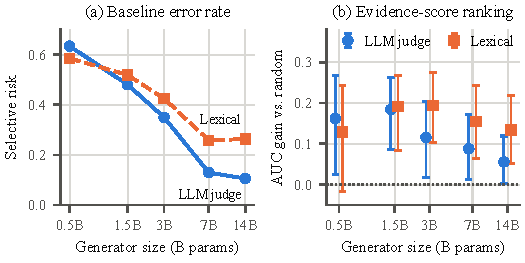
\includegraphics[width=\columnwidth]{fig_scale.pdf}
\caption{(a) Selective risk of self-refusal RAG on clean evidence. (b) Gain of the sufficiency
score's risk--coverage AUC over a random ranking, on the questions the generator answered;
bars are 95\% bootstrap intervals.}
\label{fig:scale}
\end{figure}

\subsection{Decomposing the Gain}\label{sec:decomp}
Table~\ref{tab:decomp} compares the four decision rules at 7B and 14B, and
Table~\ref{tab:ci} gives the paired differences from the unconditional baseline. ECERAG reduces
selective risk substantially and significantly on clean, irrelevant, and outdated evidence, for
both generators and both graders---for example from 0.43 to 0.13 at 7B and from 0.40 to 0.11 at
14B on clean evidence.

The decomposition shows where this gain comes from. Self-refusal alone reaches almost the same
operating point: 0.13 at 7B and 0.11 at 14B; at 14B, ECERAG and self-refusal make identical
decisions. The evidence gate alone moves the unconditional system only slightly. Its reductions
are significant under the judge for the 7B model on clean and outdated evidence and for the 14B
model on outdated evidence (Table~\ref{tab:ci}); none is significant under the lexical grader. The
gate also catches few unanswerable questions (abstention recall 0.09--0.33 versus 1.00 for
self-refusal), because false-premise questions retrieve evidence that looks relevant.
Fig.~\ref{fig:tradeoff} shows the full trade-off: sweeping the gate threshold over unconditional
answers traces a curve that lies well above the self-refusal operating point at every coverage.

\begin{table*}[t]
\caption{Selective risk / coverage (\%) by decision rule, cross-validated over 60 questions.
Upper block: LLM judge; lower block: lexical grader. Lower risk is better.}
\label{tab:decomp}
\centering
\begin{tabular}{llcccccc}
\toprule
& & \multicolumn{3}{c}{Qwen2.5-7B} & \multicolumn{3}{c}{Qwen2.5-14B}\\
\cmidrule(lr){3-5}\cmidrule(lr){6-8}
Grader & System & Clean & Irrelevant & Outdated & Clean & Irrelevant & Outdated\\
\midrule
\multirow{4}{*}{Judge}
& Unconditional RAG      & 0.43 / 100 & 0.47 / 100 & 0.63 / 100 & 0.40 / 100 & 0.38 / 100 & 0.48 / 100\\
& Evidence gate only     & 0.38 / 83  & 0.45 / 86  & 0.60 / 88  & 0.39 / 91  & 0.38 / 92  & 0.46 / 92\\
& Self-refusal RAG       & 0.13 / 52  & 0.16 / 58  & 0.36 / 54  & 0.11 / 63  & 0.03 / 62  & 0.24 / 54\\
& ECERAG                 & 0.13 / 41  & 0.14 / 41  & 0.34 / 43  & 0.11 / 63  & 0.03 / 62  & 0.24 / 54\\
\midrule
\multirow{4}{*}{Lexical}
& Unconditional RAG      & 0.52 / 100 & 0.51 / 100 & 0.57 / 100 & 0.47 / 100 & 0.40 / 100 & 0.46 / 100\\
& Evidence gate only     & 0.51 / 74  & 0.50 / 74  & 0.54 / 77  & 0.46 / 91  & 0.40 / 92  & 0.46 / 93\\
& Self-refusal RAG       & 0.26 / 52  & 0.25 / 58  & 0.40 / 54  & 0.26 / 63  & 0.21 / 62  & 0.24 / 54\\
& ECERAG                 & 0.23 / 34  & 0.20 / 35  & 0.24 / 35  & 0.30 / 53  & 0.23 / 50  & 0.26 / 47\\
\bottomrule
\end{tabular}
\end{table*}

\begin{table}[t]
\caption{Change in selective risk relative to unconditional RAG: 95\% paired bootstrap
intervals. Intervals excluding zero are in bold.}
\label{tab:ci}
\centering
\footnotesize
\setlength{\tabcolsep}{2.6pt}
\begin{tabular}{llcccc}
\toprule
& & \multicolumn{2}{c}{Evidence gate only} & \multicolumn{2}{c}{ECERAG}\\
\cmidrule(lr){3-4}\cmidrule(lr){5-6}
Model & Evidence & Judge & Lexical & Judge & Lexical\\
\midrule
7B  & Clean    & \textbf{[$-$.11,$-$.01]} & [$-$.05,.04] & \textbf{[$-$.45,$-$.16]} & \textbf{[$-$.45,$-$.14]}\\
7B  & Outdated & \textbf{[$-$.07,$-$.01]} & [$-$.06,.02] & \textbf{[$-$.47,$-$.11]} & \textbf{[$-$.50,$-$.16]}\\
14B & Clean    & [$-$.04,.02] & [$-$.04,.02] & \textbf{[$-$.42,$-$.17]} & \textbf{[$-$.32,$-$.02]}\\
14B & Outdated & \textbf{[$-$.05,$-$.00]} & [$-$.02,.03] & \textbf{[$-$.40,$-$.09]} & \textbf{[$-$.36,$-$.06]}\\
\bottomrule
\end{tabular}
\end{table}

\begin{figure}[t]
\centering
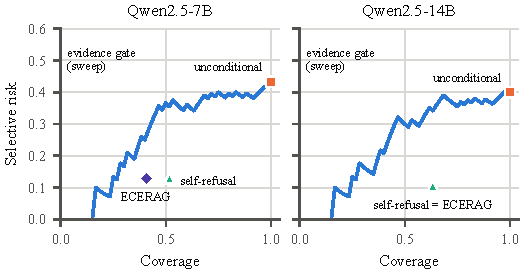
\includegraphics[width=\columnwidth]{fig_tradeoff.pdf}
\caption{Risk--coverage on clean evidence (LLM judge). The curve sweeps the evidence-gate
threshold over unconditional answers; markers are cross-validated operating points.}
\label{fig:tradeoff}
\end{figure}

\subsection{The Sufficiency Score as a Ranking Signal}\label{sec:ranking}
Although thresholding $S$ adds little to self-refusal, $S$ ranks answers well. Restricted to the
questions the generator answered (so no credit comes from its own refusals), the risk--coverage
AUC of $S$ beats a random ranking at every scale from 1.5B to 14B under both graders, with
bootstrap intervals that exclude zero, except for the 14B judge interval, whose lower bound is
0.00 (Fig.~\ref{fig:scale}b). At 7B, $S$ reaches an AUC of 0.04 against 0.13 for a random ranking
(judge; 0.10 against 0.26 lexical). Table~\ref{tab:signals} breaks the score down: relevance and
coverage carry most of the signal, trust/recency helps, and agreement is weakest on its own.

\begin{table}[t]
\caption{Risk--coverage AUC of each signal on answered questions (judge / lexical). Lower is
better; ``Random'' is the expected AUC of a random ranking.}
\label{tab:signals}
\centering
\setlength{\tabcolsep}{4pt}
\begin{tabular}{lccc}
\toprule
Score & 1.5B & 7B & 14B\\
\midrule
Random            & .48 / .52 & .13 / .26 & .11 / .26\\
$S$ (equal weights) & .30 / .33 & .04 / .10 & .05 / .13\\
$R$ relevance     & .28 / .33 & .04 / .12 & .05 / .15\\
$C$ coverage      & .26 / .29 & .05 / .09 & .05 / .14\\
$A$ agreement     & .45 / .53 & .09 / .25 & .05 / .25\\
$T$ trust/recency & .39 / .39 & .05 / .11 & .05 / .16\\
\bottomrule
\end{tabular}
\end{table}

\subsection{Contradictory Evidence and Corrective Retrieval}
The conflict check flagged all 25 contradictory evidence sets and 1 of 60 clean ones. The
check alone was the decisive fix: the pilot's agreement rule required two passages to share
\emph{no} numbers, so it could never detect a copy with one figure changed, and all systems
behaved identically under this perturbation. Acting on the flag is harder. Refusing every
flagged case yields zero risk at zero coverage. Dropping both conflicting copies recovers 38\% (7B)
and 28\% (14B) coverage, but at a selective risk of 0.27 and 0.14 (judge), not significantly
different from the unconditional baseline's 0.20 and 0.12, because the dropped pair usually
contains the passage with the answer. Self-refusal RAG remains strong on this condition (0.14 and
0.05 risk at 88\% coverage). Corrective retrieval that replaces the evidence wholesale increased
risk at 14B (0.05 to 0.23 on contradictory evidence); the merged, margin-gated version left coverage and
selective risk unchanged in every condition.

\subsection{Ablations}\label{sec:ablation}
Fitting the four weights by logistic regression, and adding an NLI-based grounding score of the
drafted answer, did not significantly improve selective risk over equal weights at 7B (judge,
95\% interval of the difference from the baseline $[-0.10,+0.03]$). The grounding score's
apparent AUC advantage disappeared once the generator's own refusals were excluded from the
ranking. Removing any single signal changed clean-condition risk by at most 0.03. With the
pilot's fixed-split calibration (17 calibration and 43 test questions), the grid selected
$\tA=0.80$ for both 7B and 14B, giving zero errors at 26\% coverage against 0.13 and 0.10 for the
baseline: a conservative operating point that the cross-validated cost function does not choose.

\section{Discussion}
\textbf{Implications.} For enterprise RAG, the most effective single control in our study is to
instruct the generator to answer only from cited evidence and to refuse otherwise, provided the
generator is large enough to follow the instruction (3B and up here). Evidence-sufficiency scores
add a calibrated, inspectable confidence signal on top of that. They are useful for ranking,
triage, and routing outdated or conflicting evidence to review, and they provide an audit trail
that self-refusal alone does not. Whether to gate on them is a risk-tolerance choice, which
Fig.~\ref{fig:tradeoff} makes explicit.

\textbf{Limitations.} The benchmark has 60 questions from six documents, so many intervals are
wide; results may not transfer to other domains without recalibration. Correctness is graded
automatically; the two graders agree on 75--82\% of answers, and we have not yet validated either
against human judgment (an annotation sheet of 100 stratified answers is released with the code).
Unanswerable questions were authored by us and may be easier to detect through self-refusal than
those arising in practice. All generators come from one model family, and the 14B model was
quantized. The perturbations are synthetic; in particular, the contradiction check targets
near-duplicate passages that disagree on a figure, which matches our injection procedure but is
only one kind of real-world conflict.

\section{Conclusion}
Enterprise RAG should move from retrieve-then-generate to retrieve--assess--decide. In a
controlled study across five generator sizes, ECERAG reduced the error rate on answered questions
by roughly two-thirds relative to unconditional RAG. Most of the reduction comes from grounded
self-refusal by the generator; the evidence-sufficiency gate adds a small, sometimes significant
improvement, and its score reliably ranks answer correctness from 1.5B to 14B parameters. Future
work will validate grading against human annotation, enlarge the benchmark, and use the
sufficiency score to drive targeted retrieval rather than blanket abstention.

\section*{Code and Data Availability}
The pipeline, corpus sources, benchmark, raw model outputs, and analysis scripts are available
at\\ \url{https://github.com/yomisys/LLM}.

\balance
\bibliographystyle{IEEEtran}
\bibliography{refs}

\end{document}
